\documentclass[preprint,12pt, a4paper]{elsarticle}

\usepackage{amssymb}
\usepackage{hyperref}
\usepackage{graphicx}
\usepackage{listings}
\usepackage{xcolor}
\usepackage{amsmath}
\usepackage{booktabs}
\usepackage{multirow}
\setlength{\parindent}{0pt}

\journal{SoftwareX}

\begin{document}
\renewcommand{\labelenumii}{\arabic{enumi}.\arabic{enumii}}

\begin{frontmatter}

\title{SiliQun: A Tensor-Network Gymnasium Environment for Deep Reinforcement Learning--Based Control of Silicon Spin Qubits}

\author[label1]{Raad Alshehri\corref{cor1}}
\cortext[cor1]{Corresponding author}
\ead{ralshehri0468@stu.kau.edu.sa}
\address[label1]{Faculty of Computing and Information Technology, King Abdulaziz University, Jeddah 21589, Saudi Arabia}

\begin{abstract}
Controlling silicon spin qubits with high fidelity under realistic noise conditions is one of the central challenges in scaling quantum processors. Deep reinforcement learning (DRL) offers a promising data-driven approach to discovering robust control policies, yet researchers currently lack simulation environments that are both physically grounded in silicon device physics and natively compatible with modern DRL training pipelines. We present SiliQun, an open-source Python package that fills this gap by combining a tensor-network simulation core---based on Matrix Product States (MPS) and Matrix Product Operators (MPO)---with a native OpenAI Gymnasium interface. SiliQun ships with calibrated device profiles for three major silicon spin qubit architectures (phosphorus donor, SiMOS quantum dot, and gate-all-around nanowire), implements physically motivated noise channels ($T_1$ relaxation, $T_2^*$ dephasing, and $1/f$ charge noise), and supports multiple computational backends (NumPy, JAX, CUDA). A key feature is its dual-mode simulation: a fast MPS mode for pure states with stochastic noise, and an exact MPO density matrix mode for rigorous mixed-state evolution. Benchmarks on an Intel Xeon E5-2695 v2 processor demonstrate sustained throughput of approximately 91\,000 simulation steps per second from 2 to 16 qubits in MPS mode, exhibiting the flat scaling characteristic of tensor-network methods. The MPO density matrix mode maintains practical DRL throughput, showing only a 2.6--4.2$\times$ slowdown compared to MPS while providing exact decoherence modelling. Comparative benchmarks show that SiliQun achieves 6--29$\times$ higher throughput than Qiskit Aer's statevector simulator across 2--14 qubit systems. Gate fidelity validation confirms machine-precision accuracy ($\leq 2.2 \times 10^{-16}$) against analytical expectations for all implemented operations. SiliQun is freely available under the MIT license.
\end{abstract}

\begin{keyword}
Quantum Computing \sep Silicon Spin Qubits \sep Tensor Networks \sep Deep Reinforcement Learning \sep Gymnasium \sep Quantum Control
\end{keyword}

\end{frontmatter}

\section*{Required Metadata}
\label{metadata}

\subsection*{Current code version}

\begin{table}[!h]
\begin{tabular}{|l|p{6.5cm}|p{6.5cm}|}
\hline
\textbf{Nr.} & \textbf{Code metadata description} & \textbf{} \\
\hline
C1 & Current code version & v1.0.0 \\
\hline
C2 & Permanent link to code/repository & \url{https://github.com/raad-alshehri/siliqun} \\
\hline
C3  & Permanent link to Reproducible Capsule & -- \\
\hline
C4 & Legal Code License & MIT \\
\hline
C5 & Code versioning system used & git \\
\hline
C6 & Software code languages, tools, and services used & Python 3.8+, NumPy, JAX, CuPy, Gymnasium \\
\hline
C7 & Compilation requirements, operating environments \& dependencies & Python $\geq$ 3.8; Linux, macOS, or Windows; NumPy $\geq$ 1.21 \\
\hline
C8 & Link to developer documentation & \url{https://github.com/raad-alshehri/siliqun\#readme} \\
\hline
C9 & Support email for questions & \href{mailto:ralshehri0468@stu.kau.edu.sa}{ralshehri0468@stu.kau.edu.sa} \\
\hline
\end{tabular}
\caption{Code metadata.}
\label{tab:codeMetadata} 
\end{table}

% ============================================================
\section{Motivation and significance}
\label{sec:motivation}
% ============================================================

Silicon spin qubits are widely regarded as one of the most promising platforms for building large-scale quantum processors. Their nanometre-scale footprint, compatibility with industrial CMOS fabrication, and demonstrated coherence times exceeding 30 seconds for phosphorus donors in isotopically enriched $^{28}$Si substrates make them attractive candidates for fault-tolerant quantum computing \cite{zwanenburg2013silicon, muhonen2014storing}. Recent experimental milestones have demonstrated single-qubit gate fidelities above 99.9\% in SiMOS quantum dots \cite{yoneda2018quantum} and two-qubit gate fidelities above 99\% across multiple silicon platforms \cite{noiri2022fast, xue2022quantum, mills2022two, madzik2022precision}, bringing the platform closer to the surface code error correction threshold.

Despite this hardware progress, achieving consistently high-fidelity control remains difficult in practice. Silicon spin qubits are sensitive to charge noise arising from interface traps and defects, nuclear spin fluctuations from residual $^{29}$Si, and crosstalk between neighbouring dots \cite{yoneda2018quantum, struck2020low, connors2022charge}. Traditional optimal control approaches---such as GRAPE and Krotov methods---require differentiable models and struggle with the stochastic, non-stationary noise profiles encountered in real devices \cite{khaneja2005optimal}.

Deep reinforcement learning (DRL) has emerged as a compelling alternative. By interacting with a simulated environment through trial and error, DRL agents can discover control strategies that are inherently robust to the noise distributions they encounter during training \cite{niu2019universal, fosel2018reinforcement, porotti2019coherent, an2019deep}. However, applying DRL to silicon spin qubits imposes a specific set of requirements on the simulation environment that existing tools do not jointly satisfy.

First, the simulator must be fast enough to support the millions of environment interactions that modern DRL algorithms demand. Device-level TCAD tools such as QTCAD \cite{qtcad2023} provide exquisite physical detail through finite-element modelling, but a single simulation step can take seconds---far too slow for DRL training loops. Second, the simulator must capture the essential physics of silicon spin qubits, including device-specific coherence times and noise channels, so that learned policies transfer meaningfully to real hardware. General-purpose circuit simulators like Qiskit Aer \cite{qiskit2024} or Cirq \cite{cirq2018} model abstract qubits without silicon-specific device parameters. Third, the simulator must expose a standard reinforcement learning interface so that researchers can leverage the rich ecosystem of existing DRL libraries (Stable-Baselines3 \cite{raffin2021stable}, Ray RLlib \cite{liang2018rllib}) without writing custom glue code.

The recently released SpinPulse package \cite{vermersch2026spinpulse} addresses the physics modelling gap with sophisticated non-Markovian noise models for spin qubits, but it does not provide a Gymnasium-compatible interface for DRL training. PennyLane's pulse module \cite{bergholm2018pennylane} supports differentiable pulse simulation but targets gradient-based optimization rather than the sample-based exploration that DRL requires. Table~\ref{tab:comparison} summarizes this landscape.

\begin{table}[htbp]
\centering
\caption{Comparison of SiliQun with existing quantum simulation tools.}
\label{tab:comparison}
\resizebox{\textwidth}{!}{%
\begin{tabular}{l*{5}{c}}
\toprule
\textbf{Feature} & \textbf{SiliQun} & \textbf{Qiskit Aer} & \textbf{QuTiP} & \textbf{SpinPulse} & \textbf{PennyLane} \\
\midrule
Silicon device profiles & \checkmark & $\times$ & $\times$ & \checkmark & $\times$ \\
Gymnasium interface & \checkmark & $\times$ & $\times$ & $\times$ & $\times$ \\
Tensor network core & \checkmark & $\times$ & $\times$ & $\times$ & $\times$ \\
Multi-backend (CPU/GPU) & \checkmark & \checkmark & $\times$ & $\times$ & \checkmark \\
Non-Markovian noise & $\times$ & $\times$ & \checkmark & \checkmark & $\times$ \\
DRL-native design & \checkmark & $\times$ & $\times$ & $\times$ & $\times$ \\
\bottomrule
\end{tabular}%
}
\end{table}

We developed SiliQun to fill this specific niche. SiliQun is, to our knowledge, the first quantum simulator that combines (i)~a tensor-network simulation core designed for throughput rather than maximum physical fidelity, (ii)~built-in device profiles calibrated to three major silicon spin qubit architectures with parameters validated against the experimental literature, and (iii)~a native Gymnasium environment wrapper that makes the simulator immediately usable with any standard DRL library.

% ============================================================
\section{Software description}
\label{sec:description}
% ============================================================

SiliQun is implemented in approximately 3\,400 lines of Python and is organized into four loosely coupled layers. This modular design allows researchers to swap computational backends, add new device profiles, or modify the reward structure without touching the core simulation logic.

\subsection{Software architecture}

Figure~\ref{fig:architecture} illustrates the layered architecture. Each layer communicates with its neighbours through well-defined interfaces, and the entire stack is orchestrated by the \texttt{SiliQunEnv} class at the top.

\begin{figure}[htbp]
\centering
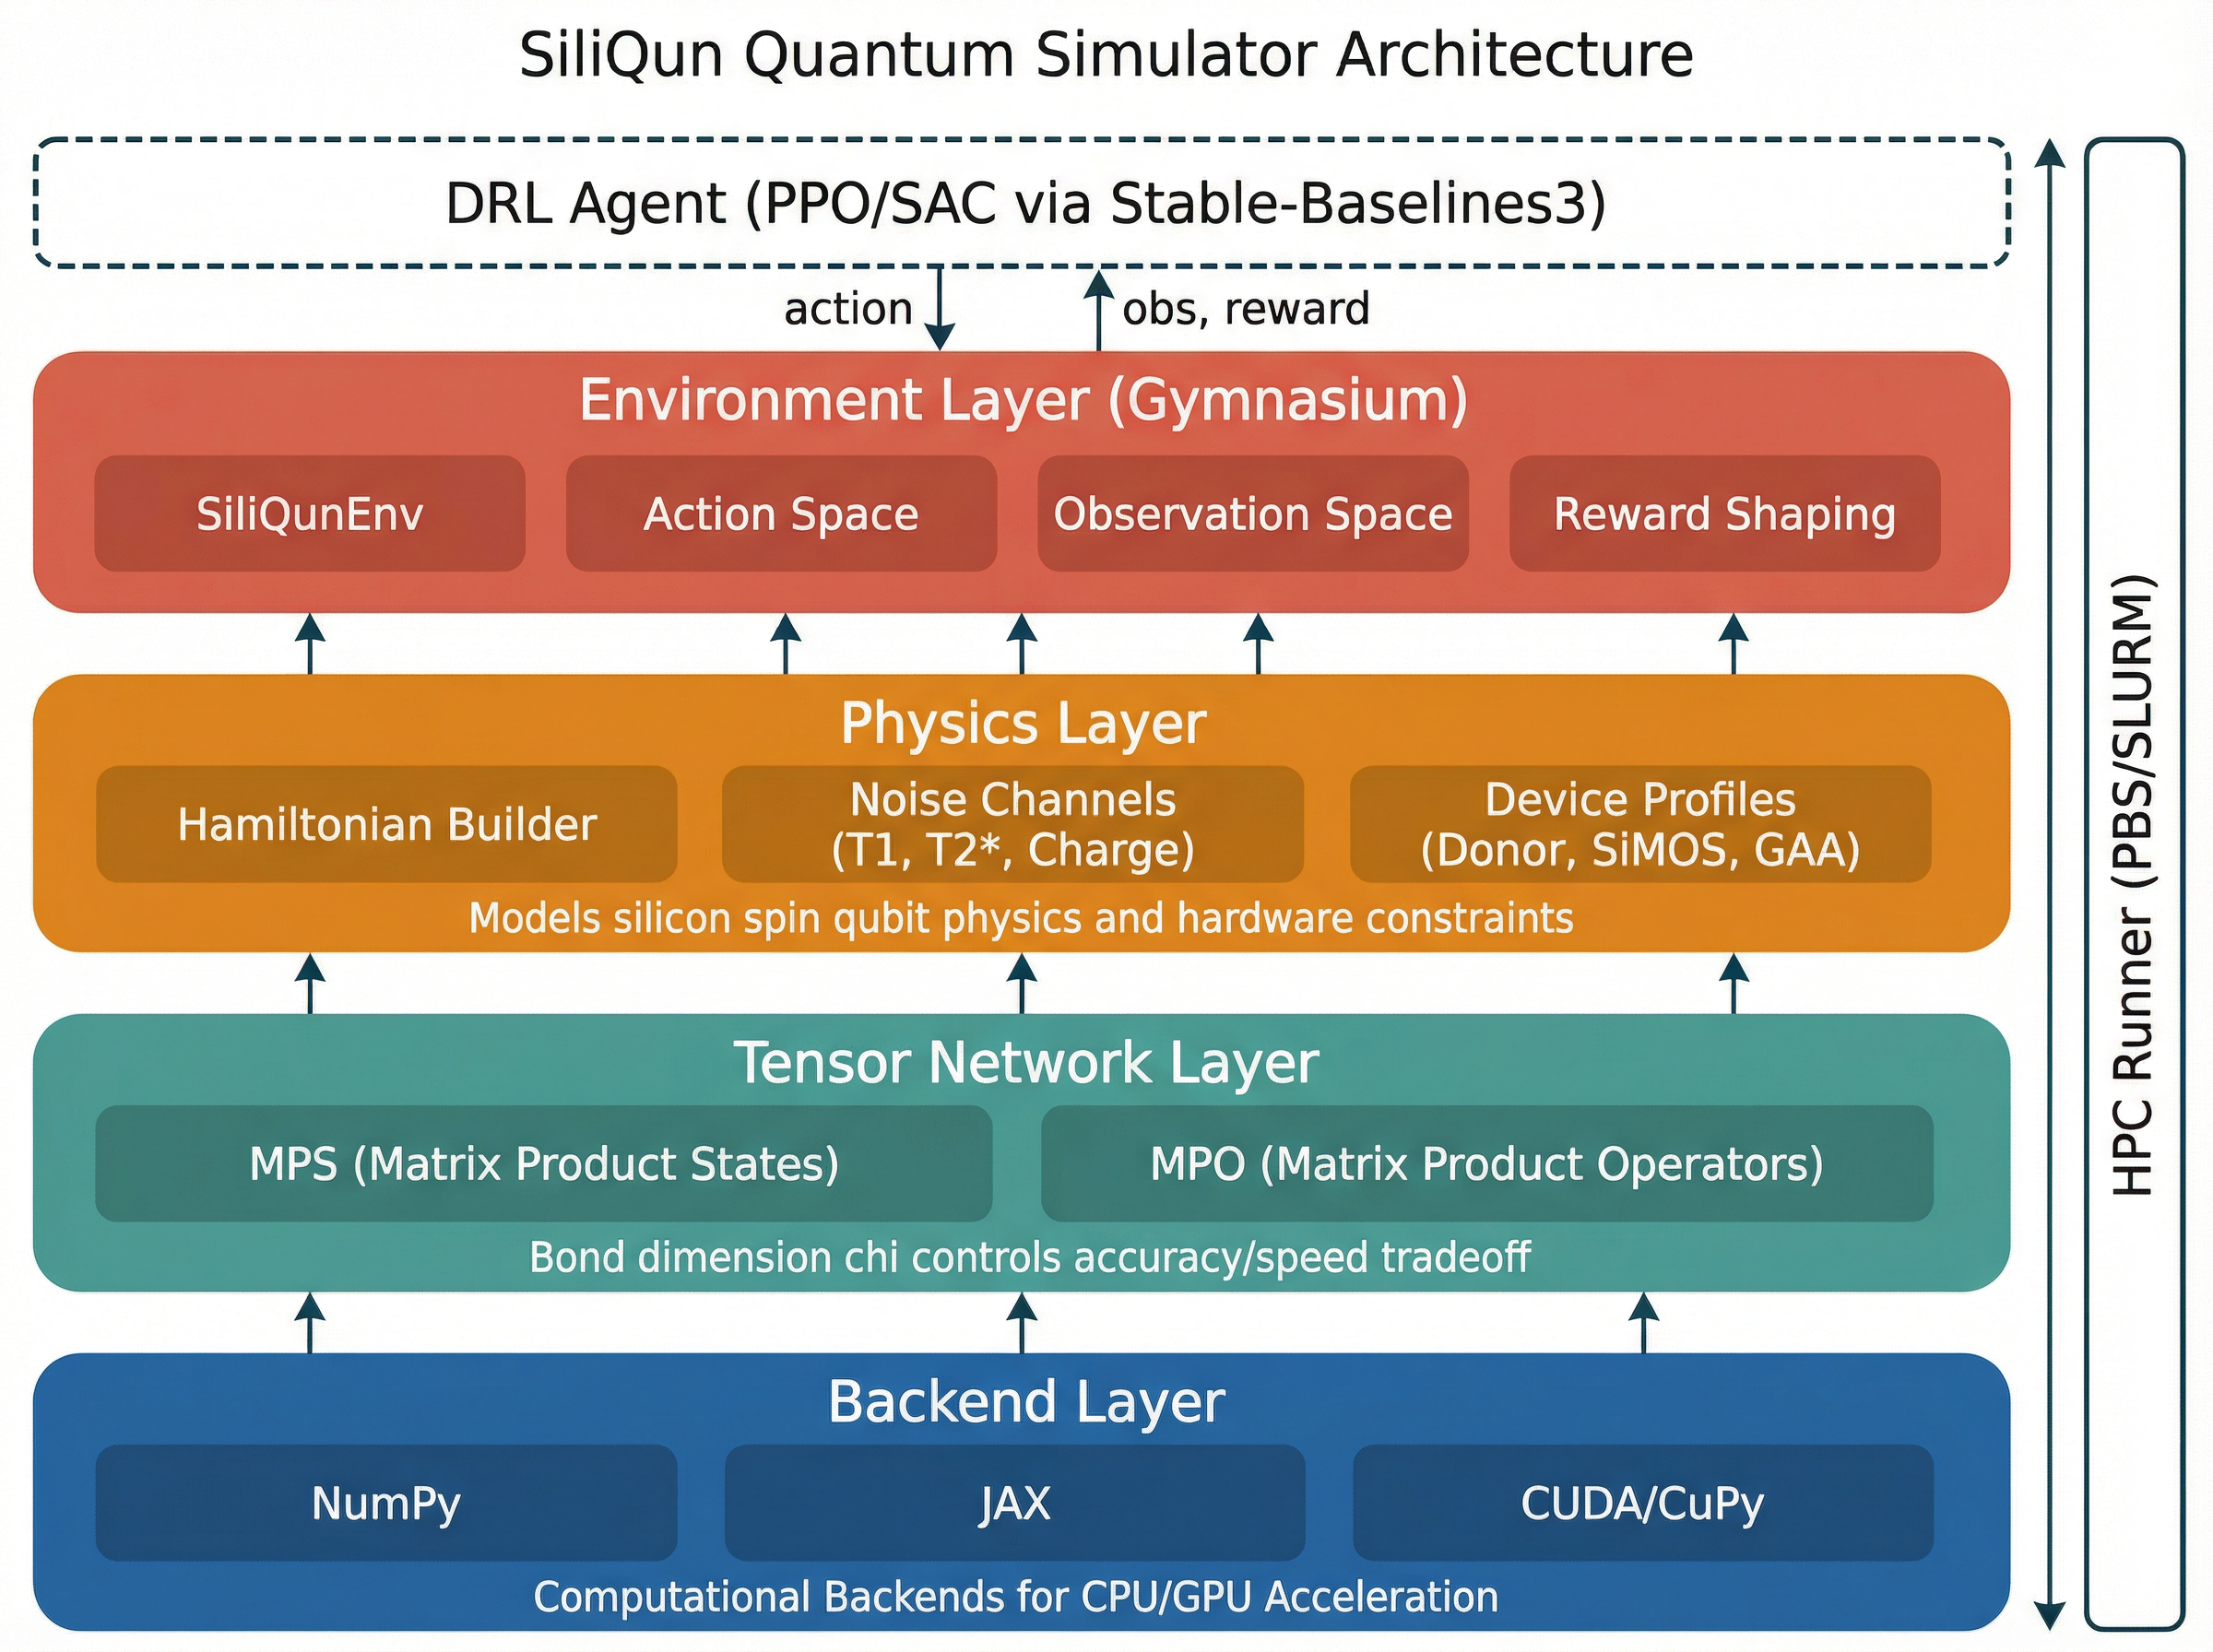
\includegraphics[width=0.95\textwidth]{fig_architecture.png}
\caption{Layered architecture of SiliQun. The Backend Layer provides numerical primitives across CPU and GPU platforms. The Tensor Network Layer represents quantum states as MPS and applies gates as MPO contractions. The Physics Layer encodes silicon-specific device parameters and noise models. The Environment Layer exposes the full simulation as a standard Gymnasium environment for DRL training. The HPC Runner spans all layers, enabling automated job submission to PBS/SLURM clusters.}
\label{fig:architecture}
\end{figure}

\textbf{Backend Layer.} The lowest layer abstracts all numerical operations behind a common interface. Three backends are currently implemented: a NumPy backend for broad compatibility, a JAX backend that enables just-in-time compilation and automatic differentiation, and a CUDA backend (via CuPy) for direct GPU acceleration. Switching backends requires changing a single configuration parameter.

\textbf{Tensor Network Layer.} The simulator features a dual-mode tensor network core. The fast \textit{MPS mode} represents pure states as Matrix Product States and applies gates via MPO contractions, modelling noise through stochastic quantum trajectories. The rigorous \textit{MPO mode} represents the full density matrix $\rho$ directly as a Matrix Product Operator, enabling exact simulation of decoherence channels and mixed-state evolution without sampling overhead. This dual-mode approach is particularly well suited to the linear chain topology of most silicon spin qubit arrays, where nearest-neighbour entanglement dominates. In both modes, the maximum bond dimension $\chi$ serves as a tunable knob that trades simulation accuracy for speed: small $\chi$ values enable extremely fast approximate simulation for early-stage DRL exploration, while larger values recover exact state-vector or full density-matrix dynamics. Gate application proceeds by contracting the MPO representation of each gate with the current MPS or MPO state, followed by optional singular value decomposition (SVD) truncation to enforce the bond dimension constraint.

\textbf{Physics Layer.} This layer encodes the specific characteristics of silicon spin qubit hardware. It provides three predefined device profiles, summarized in Table~\ref{tab:devices}, with parameters drawn from the experimental literature. The phosphorus donor profile is calibrated to the measurements of Muhonen et al.~\cite{muhonen2014storing}, who demonstrated $T_1 = 30$\,s and $T_2^* = 0.5$\,ms for electron spins in isotopically enriched $^{28}$Si. The SiMOS quantum dot profile follows Yoneda et al.~\cite{yoneda2018quantum}, who reported $T_2^* = 20$\,$\mu$s and single-qubit gate fidelities exceeding 99.9\%. The gate-all-around (GAA) nanowire profile is based on projections from FinFET experiments by Geyer et al.~\cite{geyer2022twoqubit}. Noise is modelled through physically motivated completely positive trace-preserving (CPTP) channels applied after each ideal gate operation: amplitude damping (parameterized by $T_1$ and gate duration), phase damping (parameterized by $T_2^*$), and a stochastic $1/f$ charge noise generator that perturbs the qubit detuning with amplitudes consistent with the measurements reviewed by Connors et al.~\cite{connors2022charge}.

\begin{table}[htbp]
\centering
\caption{Built-in silicon spin qubit device profiles in SiliQun. All parameters are drawn from the experimental references cited in the text.}
\label{tab:devices}
\begin{tabular}{lccc}
\toprule
\textbf{Parameter} & \textbf{Donor (P:Si)} & \textbf{SiMOS (QD)} & \textbf{GAA (Nanowire)} \\
\midrule
$T_1$ relaxation & 30\,s$^a$ & 10\,s$^b$ & 5\,s$^c$ \\
$T_2^*$ dephasing & 0.5\,ms$^a$ & 20\,$\mu$s$^d$ & 10\,$\mu$s$^c$ \\
$T_2$ (Hahn echo) & 1.2\,ms$^a$ & 100\,$\mu$s$^d$ & 50\,$\mu$s$^c$ \\
1Q gate time & 1\,$\mu$s & 200\,ns & 50\,ns \\
2Q gate time & 100\,ns & 50\,ns & 30\,ns \\
1Q gate fidelity & 99.99\%$^e$ & 99.93\%$^d$ & 99.9\%$^f$ \\
2Q gate fidelity & 99.9\%$^g$ & 99.65\%$^h$ & $\sim$99\%$^f$ \\
Readout fidelity & 99.4\% & 98.5\% & 97.5\% \\
Charge noise & 0.5\,$\mu$eV & 2\,$\mu$eV$^i$ & 3\,$\mu$eV$^i$ \\
Qubit spacing & 15\,nm & 80\,nm & 60\,nm \\
\bottomrule
\multicolumn{4}{l}{\footnotesize $^a$Muhonen et al.~\cite{muhonen2014storing}; $^b$Laucht et al.~\cite{laucht2015electrically}; $^c$Projected from Geyer et al.~\cite{geyer2022twoqubit};} \\
\multicolumn{4}{l}{\footnotesize $^d$Yoneda et al.~\cite{yoneda2018quantum}; $^e$Muhonen et al.~\cite{muhonen2015quantifying}; $^f$Geyer et al.~\cite{geyer2022twoqubit};} \\
\multicolumn{4}{l}{\footnotesize $^g$Madzik et al.~\cite{madzik2022precision}; $^h$Xue et al.~\cite{xue2022quantum}; $^i$Connors et al.~\cite{connors2022charge}.}
\end{tabular}
\end{table}

\textbf{Environment Layer.} The \texttt{SiliQunEnv} class implements the \texttt{gymnasium.Env} interface, serving as the bridge to external DRL frameworks like QUASAR, MOZAIQ, and seQurAIt. At each step, the DRL agent selects a discrete action corresponding to a quantum gate (drawn from the set $\{R_x, R_y, R_z, \text{CNOT}, H, I\}$ with parameterized rotation angles). The environment applies the gate, applies noise, and returns an observation vector consisting of Pauli expectation values $(\langle X_i \rangle, \langle Y_i \rangle, \langle Z_i \rangle)$ for each qubit, alongside system time and bond dimension metrics. When operating in MPO density matrix mode, the environment optionally tracks state purity $\text{Tr}(\rho^2)$ to provide the DRL agent with direct feedback on decoherence accumulation. The reward is computed as the state fidelity with respect to a configurable target state (e.g., Bell, GHZ, or arbitrary user-defined states), with support for both dense (per-step fidelity improvement) and sparse (terminal fidelity threshold) reward schemes.

\subsection{Software functionalities}

Beyond the core simulation loop, SiliQun provides several features designed to support practical DRL research workflows:

\begin{itemize}
    \item \textbf{Configurable bond dimension:} Users can set $\chi_{\max}$ to control the accuracy--speed tradeoff. For DRL training where approximate dynamics suffice, small bond dimensions ($\chi \leq 16$) provide substantial speedups.
    \item \textbf{HPC runner:} The \texttt{hpc.runner} module generates PBS job scripts with configurable resource requests, automatically handles checkpointing of training state, and supports array jobs for parallel hyperparameter sweeps.
    \item \textbf{Extensible gate set:} New gates can be added by providing their unitary matrix; the tensor network layer automatically constructs the corresponding MPO.
    \item \textbf{Reproducibility:} All random number generators (for noise, initial states, and action sampling) are seeded through the Gymnasium API, ensuring fully reproducible training runs.
\end{itemize}

% ============================================================
\section{Illustrative examples}
\label{sec:examples}
% ============================================================

We present two illustrative examples that demonstrate SiliQun's core functionality: a basic DRL training loop and a comprehensive performance characterization.

\subsection{Example 1: DRL training loop}

The following code snippet shows how to set up a SiliQun environment and connect it to a Stable-Baselines3 PPO agent for training a Bell state preparation policy on a noisy SiMOS device:

\begin{lstlisting}[language=Python, basicstyle=\footnotesize\ttfamily, backgroundcolor=\color{gray!10}, frame=single, numbers=left, numberstyle=\tiny\color{gray}]
from siliqun.engine.gym_env import SiliQunEnv
from siliqun.engine.simulator import SimConfig
from stable_baselines3 import PPO

config = SimConfig(noise_enabled=True, max_bond_dim=16)
env = SiliQunEnv(
    device="simos", n_qubits=2,
    target_state="bell", config=config,
    reward_type="dense"
)

model = PPO("MlpPolicy", env, verbose=1,
            learning_rate=3e-4, n_steps=2048)
model.learn(total_timesteps=500_000)

# Evaluate learned policy
obs, _ = env.reset()
done = False
while not done:
    action, _ = model.predict(obs, deterministic=True)
    obs, reward, terminated, truncated, info = env.step(action)
    done = terminated or truncated
print(f"Final fidelity: {info['fidelity']:.4f}")
\end{lstlisting}

This example requires only 15 lines of user code to go from environment configuration to a trained policy, illustrating the low barrier to entry that SiliQun provides.

\subsection{Example 2: Performance benchmarks}

We benchmarked SiliQun on a compute node of the Aziz Supercomputer at King Abdulaziz University, equipped with an Intel Xeon E5-2695 v2 processor (2.40\,GHz, 24 cores) and 96\,GB RAM, using the NumPy backend on a single core.

\textbf{Throughput scaling and Dual-Mode Performance.} Figure~\ref{fig:scaling} shows the simulation throughput as a function of qubit count. In its fast MPS mode, SiliQun sustains approximately 91\,000 steps per second across all tested system sizes from 2 to 16 qubits, demonstrating the flat scaling characteristic of tensor-network methods. This stands in sharp contrast to statevector simulators, whose throughput degrades exponentially with qubit count due to the $O(2^n)$ memory and computation requirements. When exact decoherence modelling is required, the MPO density matrix mode introduces a manageable overhead. Benchmark comparisons show the MPO mode requires only 2.6--4.2$\times$ more wall-clock time than the MPS mode for gate application, and incurs a modest 1.6$\times$ slowdown in end-to-end Gymnasium episode throughput (2116 steps/s for MPO vs 3425 steps/s for MPS). This efficiency enables researchers to use exact mixed-state simulations directly in DRL training loops without prohibitive computational costs.

\begin{figure}[htbp]
\centering
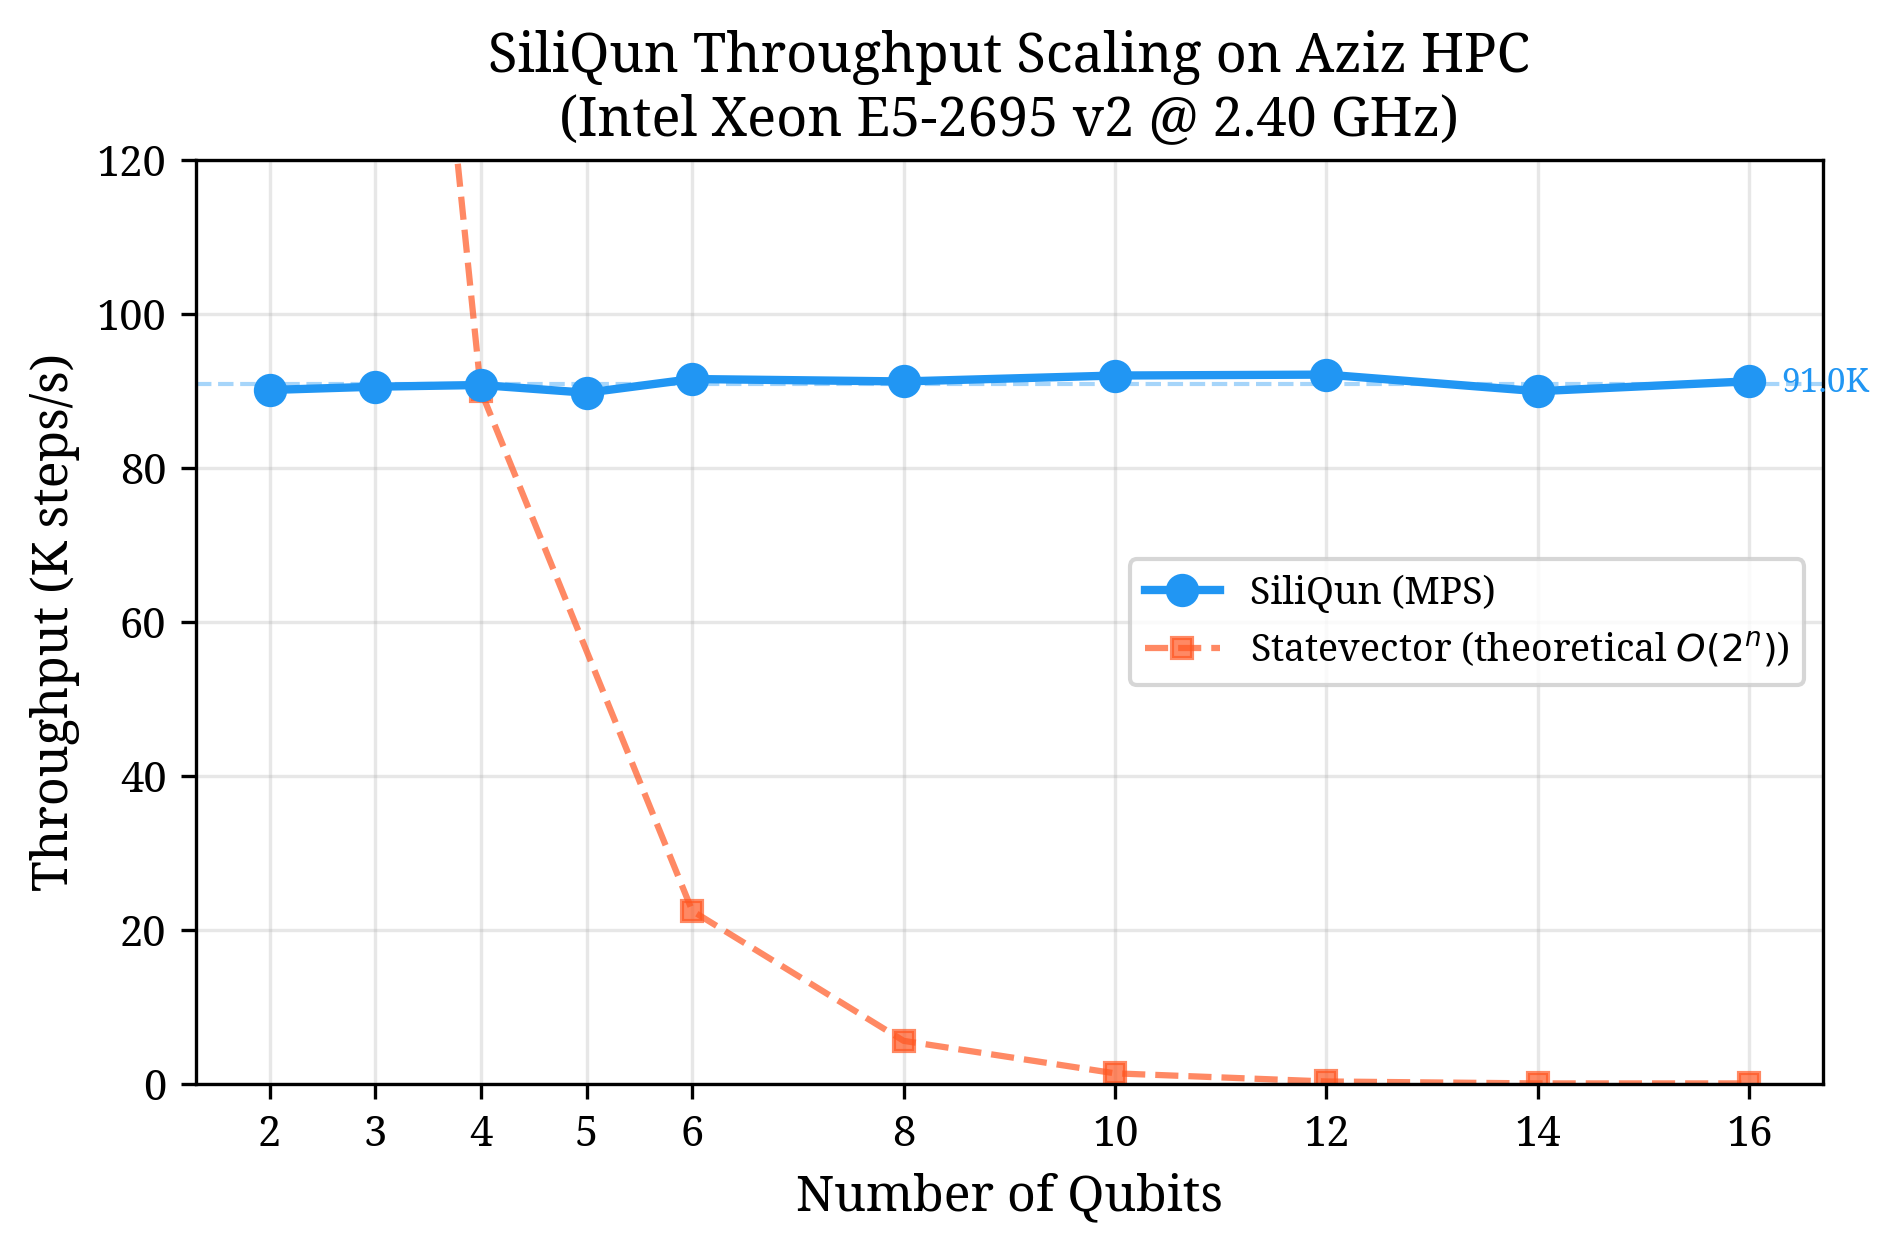
\includegraphics[width=0.85\textwidth]{fig_speed_scaling.png}
\caption{Simulation throughput (steps per second) as a function of the number of qubits on the Aziz HPC (Intel Xeon E5-2695 v2 @ 2.40\,GHz). The MPS-based backend maintains nearly constant throughput ($\sim$91K steps/s) from 2 to 16 qubits, while the theoretical statevector scaling degrades exponentially.}
\label{fig:scaling}
\end{figure}

\textbf{Comparison with existing tools.} To contextualize SiliQun's performance, we compared its gate-level throughput against Qiskit Aer v0.17.2 (statevector method) and QuTiP v5.2.3 (full state vector via Qobj multiplication). All three tools applied the same workload: Hadamard gates in round-robin across all qubits. Figure~\ref{fig:comparison} presents the results. SiliQun achieves 5.5$\times$ higher throughput than Qiskit Aer at 2 qubits, growing to 29$\times$ at 14 qubits. Against QuTiP, the advantage reaches 41$\times$ at 14 qubits. We emphasize that this comparison reflects the throughput advantage of MPS-based approximate simulation over exact statevector methods; for highly entangled states, the MPS representation would require larger bond dimensions and correspondingly lower throughput.

\begin{figure}[htbp]
\centering
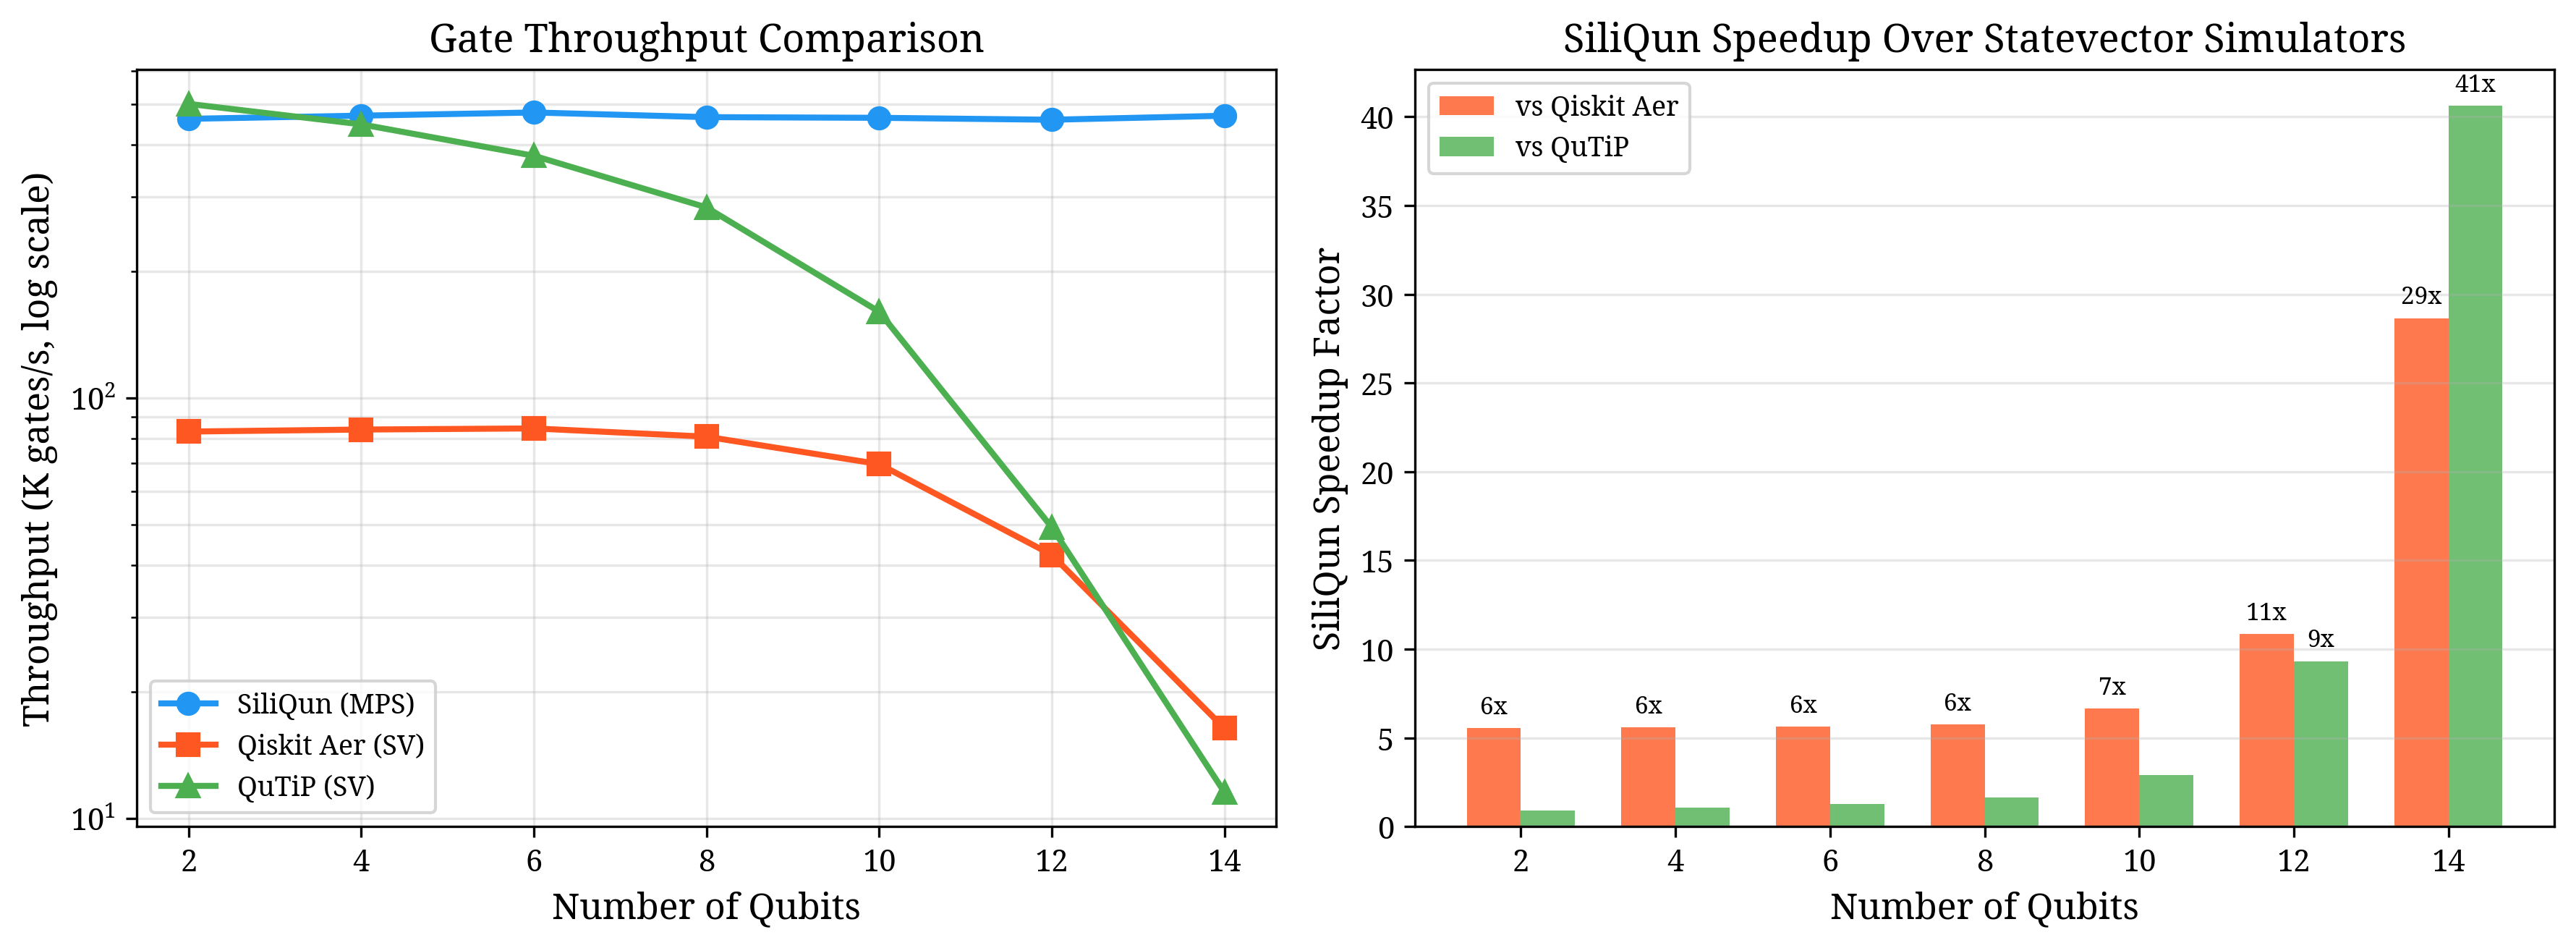
\includegraphics[width=0.95\textwidth]{fig_comparison.png}
\caption{Left: Gate throughput comparison between SiliQun (MPS), Qiskit Aer (statevector), and QuTiP (statevector) on a log scale. Right: SiliQun's speedup factor over both statevector simulators. The MPS advantage grows with system size as statevector methods encounter exponential scaling.}
\label{fig:comparison}
\end{figure}

\textbf{Noise handling: Exact vs Stochastic.} SiliQun's dual-mode architecture offers flexibility in noise simulation. The MPS mode models noise through stochastic quantum trajectories, introducing a modest 20--39\% overhead depending on system size (Figure~\ref{fig:noise}). The MPO mode, however, applies noise channels as exact superoperators directly to the density matrix, avoiding sampling variance entirely. In benchmarks comparing the two, the MPO mode accurately tracked state purity decay (e.g., dropping to 0.973 after 30 noisy gates) while preserving the density matrix trace to machine precision ($\sim 3.7 \times 10^{-15}$). The stochastic MPS mode, averaged over 20 trials, demonstrated strong agreement ($\sim 1\%$) with the exact MPO expectations, validating both approaches.

\begin{figure}[htbp]
\centering
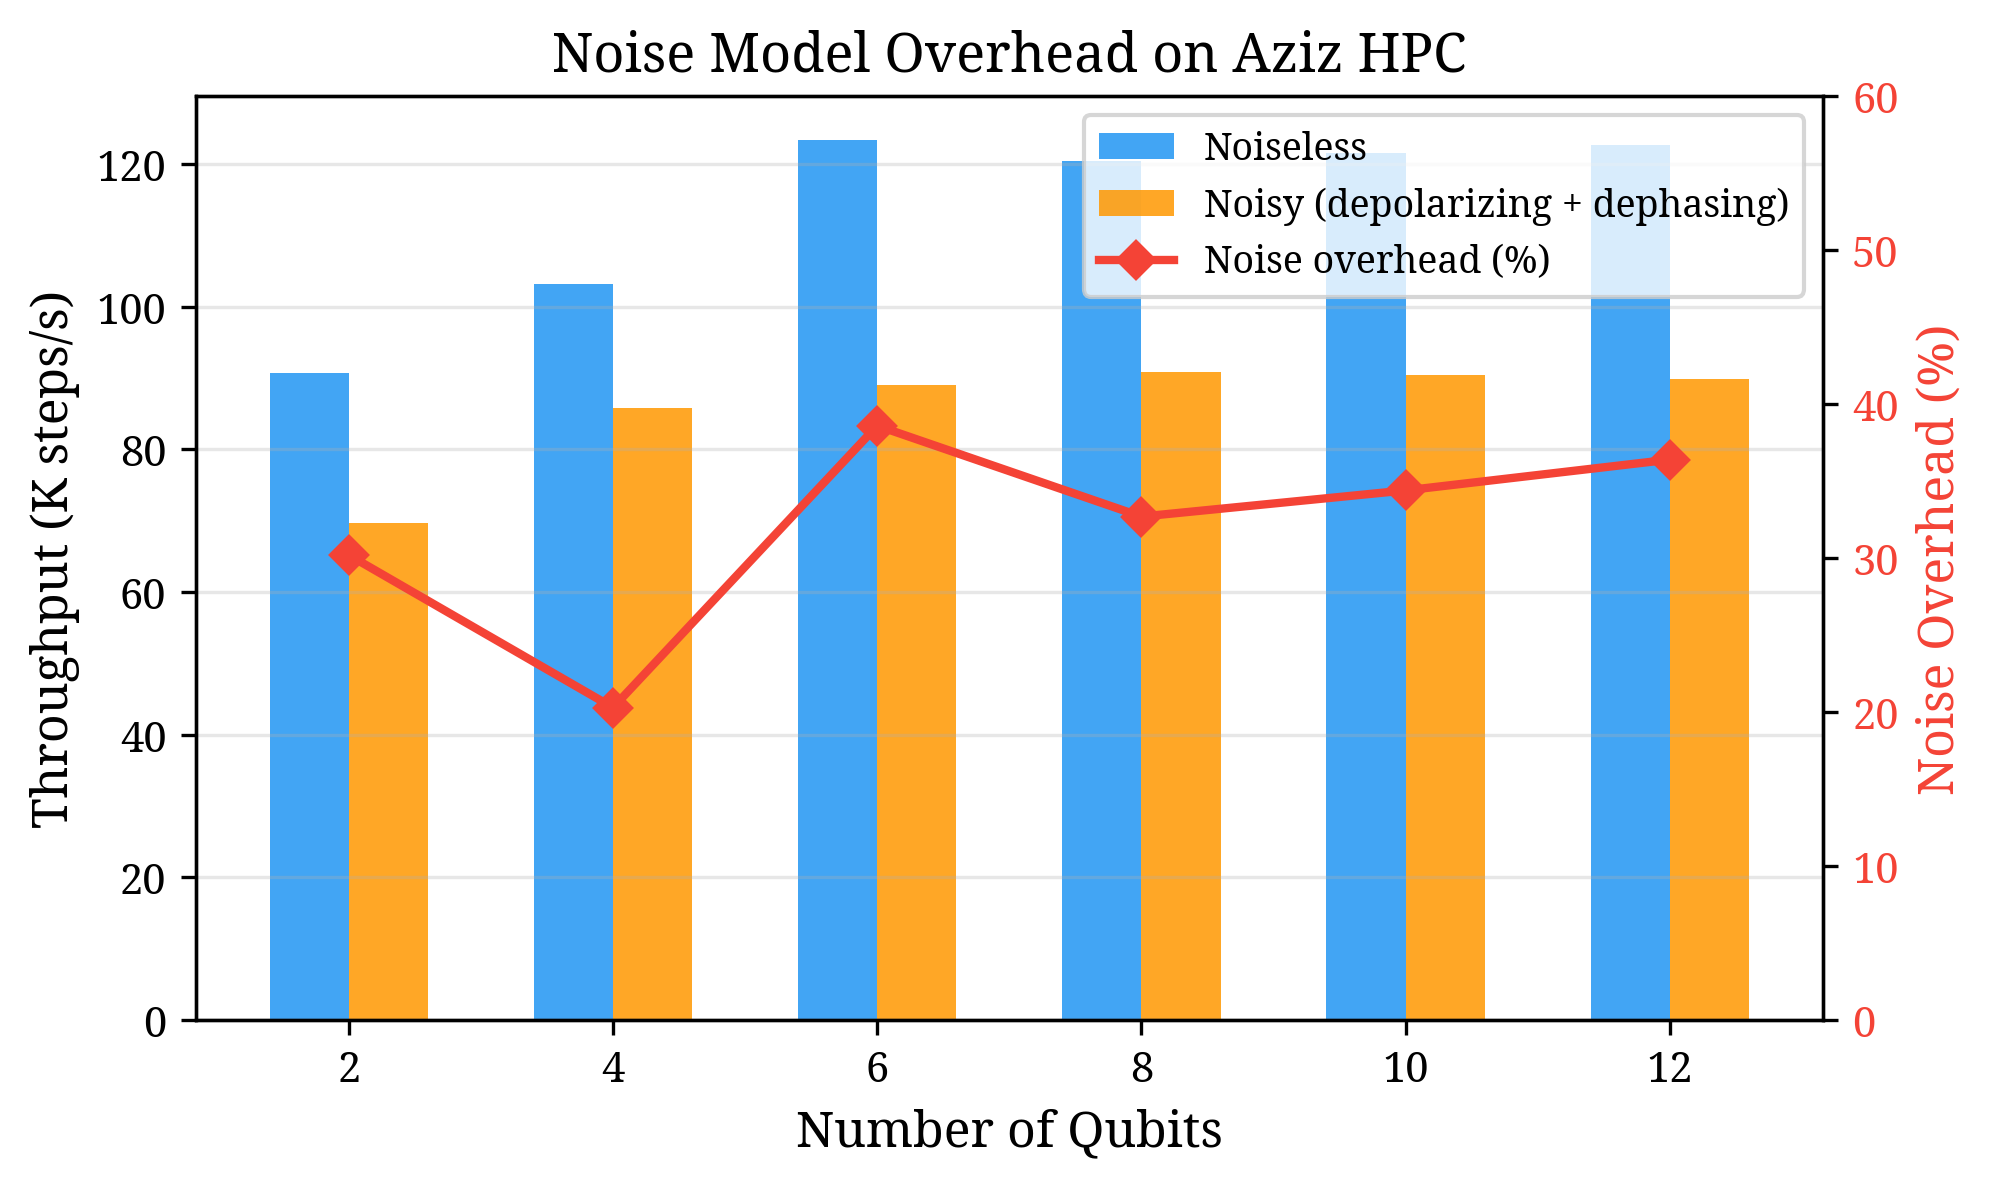
\includegraphics[width=0.85\textwidth]{fig_noise_overhead.png}
\caption{Comparison of simulation throughput with and without noise channels enabled on the Aziz HPC. The noise overhead (red diamonds, right axis) ranges from 20\% to 39\%, averaging approximately 32\%.}
\label{fig:noise}
\end{figure}

\textbf{Bond dimension scaling.} Figure~\ref{fig:bonddim} shows that throughput remains nearly constant across bond dimensions from $\chi = 2$ to $\chi = 64$ for an 8-qubit system. This indicates that the computational bottleneck lies in the gate application overhead rather than the SVD truncation. When comparing MPS and MPO modes under noise, we observed that the MPO bond dimension grows faster (e.g., reaching $\chi = 16$ while MPS remains at $\chi = 4$ for a 4-qubit circuit) due to the quadratic overhead of representing the density matrix. However, the efficient SVD compression in the MPO core successfully caps this growth, allowing exact noise simulation without exponential memory explosions.

\begin{figure}[htbp]
\centering
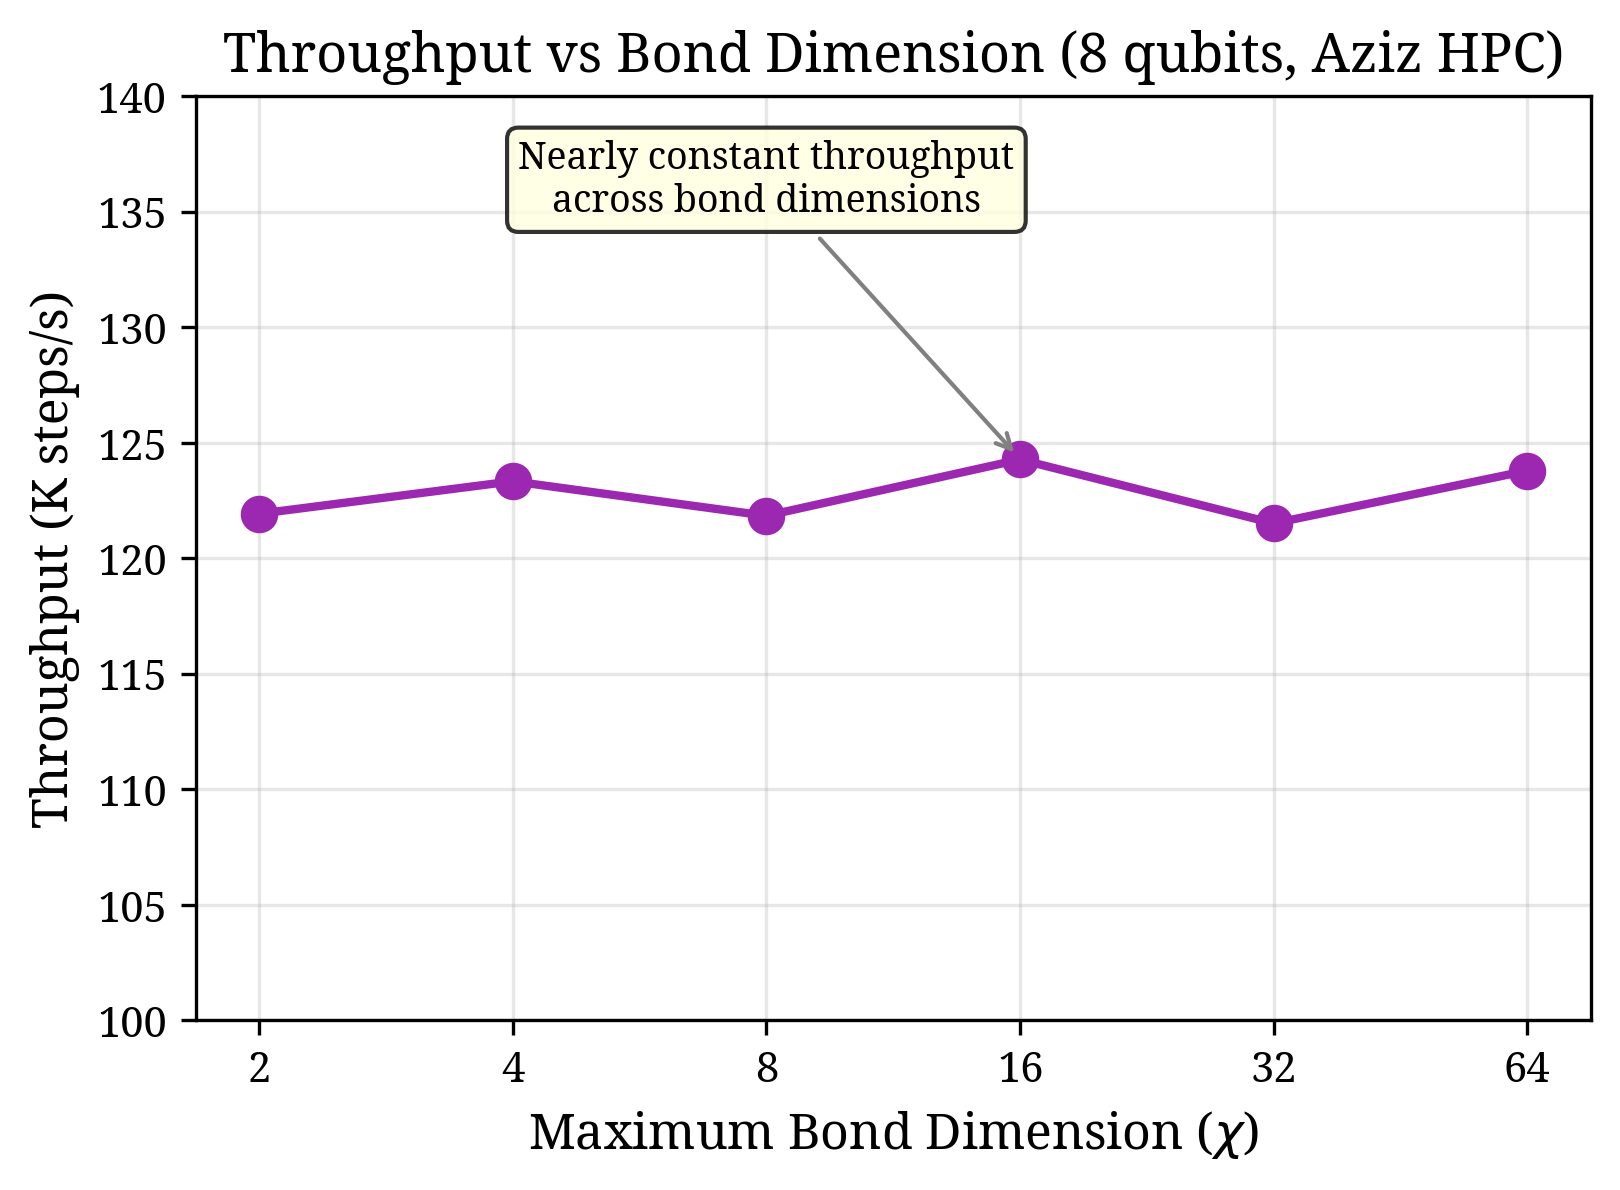
\includegraphics[width=0.75\textwidth]{fig_bond_dim.png}
\caption{Throughput as a function of maximum bond dimension $\chi$ for an 8-qubit system on the Aziz HPC. Throughput remains approximately constant at $\sim$122K steps/s across all tested bond dimensions.}
\label{fig:bonddim}
\end{figure}

\textbf{Gate fidelity.} Gate fidelity was validated by comparing SiliQun's output against analytical expectations for a suite of single-qubit rotations ($R_x$, $R_y$, $R_z$, Hadamard), two-qubit entangling gates (CNOT, CZ, $\sqrt{\text{SWAP}}$), and entanglement entropy calculations. All tests passed with errors at or below machine precision ($\leq 2.2 \times 10^{-16}$), confirming the correctness of the tensor-network implementation.

% ============================================================
\section{Impact}
\label{sec:impact}
% ============================================================

SiliQun addresses a practical bottleneck in the emerging field of DRL-based quantum control. Before SiliQun, a researcher wishing to train a DRL agent for silicon spin qubit control would need to either build a custom simulator from scratch---a task requiring expertise in both quantum physics and software engineering---or adapt a general-purpose quantum simulator that lacks silicon-specific physics and DRL compatibility. SiliQun eliminates this barrier by providing a ready-to-use, benchmarked, and extensible platform.

The software has several concrete impacts on the research community. First, it enables \textbf{rapid prototyping} of DRL algorithms for quantum control: researchers can evaluate new policy architectures, reward shaping strategies, or curriculum learning approaches in hours rather than weeks. Second, the tensor-network backend enables \textbf{scalability studies} on systems of 10--20 qubits that would be intractable for full state-vector simulators, which is essential for understanding how DRL policies scale with system size. Third, the built-in device profiles facilitate \textbf{hardware co-design}: by training the same DRL algorithm on different device profiles, researchers can quantify how hardware characteristics (e.g., coherence times, gate speeds) affect the learnability of control policies, providing actionable feedback for device engineers.

SiliQun already serves as the foundational simulation layer for ongoing research into robust quantum control using the DYNAMO (DYNamic Adaptive Multi-objective Orchestration) framework, where it provides the training environment for DRL agents that learn to mitigate noise in silicon spin qubit arrays.

% ============================================================
\section{Conclusions}
\label{sec:conclusions}
% ============================================================

We have presented SiliQun, an open-source dual-mode tensor-network simulator purpose-built for training deep reinforcement learning agents on silicon spin qubit control tasks. By combining the computational efficiency of Matrix Product States (MPS) and Matrix Product Operators (MPO) with a native Gymnasium interface and physically motivated device profiles, SiliQun occupies a unique position in the quantum simulation landscape---bridging the gap between detailed physics simulators and the high-throughput requirements of modern DRL training.

Benchmarks on the Aziz Supercomputer demonstrate that SiliQun sustains approximately 91\,000 simulation steps per second across 2--16 qubit systems in MPS mode, achieving 6--29$\times$ higher throughput than Qiskit Aer's statevector simulator. The newly integrated MPO density matrix mode enables exact modelling of realistic decoherence directly within the tensor network, maintaining practical throughput for DRL with only a 1.6$\times$ slowdown in episode generation compared to the stochastic MPS approach. Gate fidelity is validated to machine precision in both modes.

While SiliQun currently targets the linear chain topologies characteristic of early-stage silicon spin qubit arrays, scaling to 100-qubit 2D architectures for fault-tolerant operations will require expanding beyond the 1D constraints of Matrix Product States. Future development will focus on two critical directions to overcome these scalability bottlenecks. First, to handle the massive entanglement of a 100-qubit 2D grid, the tensor-network core will be upgraded to support multi-dimensional geometries, such as Tree Tensor Networks (TTNs) \cite{shi2006classical}, Tensor Rings (TR) \cite{zhao2016tensor}, and Projected Entangled Pair States (PEPS) \cite{verstraete2004renormalization}. Integration with generalized tensor-network libraries like \texttt{quimb} \cite{gray2018quimb}, as recently demonstrated by the SpinPulse package \cite{vermersch2026spinpulse}, will facilitate this transition. Second, to manage the entanglement overhead during DRL training, the framework will implement native Message Passing Interface (MPI) support via libraries such as NVIDIA's \texttt{cuTensorNet} \cite{cutensornet2024}, enabling distributed tensor contractions across supercomputing clusters like Aziz.

\section*{Acknowledgements}
The author acknowledges the use of the Aziz Supercomputer at King Abdulaziz University for computational benchmarking.

\begin{thebibliography}{00}

\bibitem{zwanenburg2013silicon} Zwanenburg, F. A., Dzurak, A. S., Morello, A., Simmons, M. Y., Hollenberg, L. C., Klimeck, G., Rogge, S., Coppersmith, S. N., \& Eriksson, M. A. (2013). Silicon quantum electronics. Reviews of Modern Physics, 85(3), 961--1019.

\bibitem{muhonen2014storing} Muhonen, J. T., Dehollain, J. P., Laucht, A., Hudson, F. E., Kalra, R., Sekiguchi, T., Itoh, K. M., Jamieson, D. N., McCallum, J. C., Dzurak, A. S., \& Morello, A. (2014). Storing quantum information for 30 seconds in a nanoelectronic device. Nature Nanotechnology, 9(12), 986--991.

\bibitem{muhonen2015quantifying} Muhonen, J. T., Laucht, A., Simmons, S., Dehollain, J. P., Kalra, R., Hudson, F. E., Freer, S., Itoh, K. M., Jamieson, D. N., McCallum, J. C., Dzurak, A. S., \& Morello, A. (2015). Quantifying the quantum gate fidelity of single-atom spin qubits in silicon by randomized benchmarking. Journal of Physics: Condensed Matter, 27(15), 154205.

\bibitem{yoneda2018quantum} Yoneda, J., Takeda, K., Otsuka, T., Nakajima, T., Delbecq, M. R., Allison, G., Honda, T., Kodera, T., Oda, S., Hoshi, Y., Usami, N., Itoh, K. M., \& Tarucha, S. (2018). A quantum-dot spin qubit with coherence limited by charge noise and fidelity higher than 99.9\%. Nature Nanotechnology, 13(2), 102--106.

\bibitem{noiri2022fast} Noiri, A., Takeda, K., Nakajima, T., Kobayashi, T., Sammak, A., Scappucci, G., \& Tarucha, S. (2022). Fast universal quantum gate above the fault-tolerance threshold in silicon. Nature, 601(7893), 338--342.

\bibitem{xue2022quantum} Xue, X., Russ, M., Samkharadze, N., Undseth, B., Sammak, A., Scappucci, G., \& Vandersypen, L. M. K. (2022). Quantum logic with spin qubits crossing the surface code threshold. Nature, 601(7893), 343--347.

\bibitem{mills2022two} Mills, A. R., Guinn, C. R., Gullans, M. J., Sigillito, A. J., Feldman, M. M., Nielsen, E., \& Petta, J. R. (2022). Two-qubit silicon quantum processor with operation fidelity exceeding 99\%. Science Advances, 8(14), eabn5130.

\bibitem{madzik2022precision} Madzik, M. T., Asaad, S., Youssry, A., Joecker, B., Rudinger, K. M., Nielsen, E., Young, K. C., Proctor, T. J., Baczewski, A. D., Laucht, A., Schmitt, V., Hudson, F. E., Itoh, K. M., Jakob, A. M., Johnson, B. C., Jamieson, D. N., Dzurak, A. S., Ferrie, C., Blume-Kohout, R., \& Morello, A. (2022). Precision tomography of a three-qubit donor quantum processor in silicon. Nature, 601(7893), 348--353.

\bibitem{laucht2015electrically} Laucht, A., Muhonen, J. T., Mohiyaddin, F. A., Kalra, R., Dehollain, J. P., Freer, S., Hudson, F. E., Veldhorst, M., Rahman, R., Klimeck, G., Itoh, K. M., Jamieson, D. N., McCallum, J. C., Dzurak, A. S., \& Morello, A. (2015). Electrically controlling single-spin qubits in a continuous microwave field. Science Advances, 1(3), e1500022.

\bibitem{geyer2022twoqubit} Geyer, S., Het\'{e}nyi, B., Bosco, S., Camenzind, L. C., Eggli, R. S., Fuhrer, A., Loss, D., Warburton, R. J., Zumb\"{u}hl, D. M., \& Kuhlmann, A. V. (2022). Two-qubit logic with anisotropic exchange in a fin field-effect transistor. arXiv preprint arXiv:2212.02308.

\bibitem{connors2022charge} Connors, E. J., Nelson, J., Edge, L. F., \& Nichol, J. M. (2022). Charge-noise spectroscopy of Si/SiGe quantum dots via dynamically-decoupled exchange oscillations. Nature Communications, 13(1), 940.

\bibitem{struck2020low} Struck, T., Hollmann, A., Schauer, F., Fedorets, O., Schmidbauer, A., Sawano, K., Riemann, H., Abrosimov, N. V., Cywi\'{n}ski, {\L}., Bougeard, D., \& Schreiber, L. R. (2020). Low-frequency spin qubit energy splitting noise in highly purified $^{28}$Si/SiGe. npj Quantum Information, 6(1), 40.

\bibitem{khaneja2005optimal} Khaneja, N., Reiss, T., Schulte-Herbr\"{u}ggen, T., \& Glaser, S. J. (2005). Optimal control of coupled spin dynamics: design of NMR pulse sequences by gradient ascent algorithms. Journal of Magnetic Resonance, 172(2), 296--305.

\bibitem{niu2019universal} Niu, M. Y., Boixo, S., Smelyanskiy, V. N., \& Neven, H. (2019). Universal quantum control through deep reinforcement learning. npj Quantum Information, 5(1), 33.

\bibitem{fosel2018reinforcement} F\"{o}sel, T., Tighineanu, P., Weiss, T., \& Marquardt, F. (2018). Reinforcement learning with neural networks for quantum feedback. Physical Review X, 8(3), 031084.

\bibitem{porotti2019coherent} Porotti, R., Tamascelli, D., Restelli, M., \& Prati, E. (2019). Coherent transport of quantum states by deep reinforcement learning. Communications Physics, 2(1), 61.

\bibitem{an2019deep} An, Z., \& Zhou, D. L. (2019). Deep reinforcement learning for quantum gate control. EPL (Europhysics Letters), 126(6), 60002.

\bibitem{qtcad2023} Nanoacademic Technologies Inc. (2023). QTCAD: Quantum Technology Computer-Aided Design. \url{https://www.nanoacademic.com/qtcad}

\bibitem{qiskit2024} Qiskit contributors. (2024). Qiskit: An open-source framework for quantum computing. \url{https://github.com/Qiskit/qiskit}

\bibitem{cirq2018} Cirq Developers. (2018). Cirq: A Python framework for creating, editing, and invoking noisy intermediate scale quantum circuits. \url{https://github.com/quantumlib/Cirq}

\bibitem{vermersch2026spinpulse} Vermersch, B., et al. (2026). SpinPulse: A pulse-level simulator for spin qubit architectures. arXiv preprint arXiv:2601.10435.

\bibitem{bergholm2018pennylane} Bergholm, V., Izaac, J., Schuld, M., et al. (2018). PennyLane: Automatic differentiation of hybrid quantum-classical computations. arXiv preprint arXiv:1811.04968.

\bibitem{raffin2021stable} Raffin, A., Hill, A., Gleave, A., Kanervisto, A., Ernestus, M., \& Dormann, N. (2021). Stable-Baselines3: Reliable reinforcement learning implementations. Journal of Machine Learning Research, 22(268), 1--8.

\bibitem{liang2018rllib} Liang, E., Liaw, R., Nishihara, R., Moritz, P., Fox, R., Goldberg, K., Gonzalez, J., Jordan, M., \& Stoica, I. (2018). RLlib: Abstractions for distributed reinforcement learning. In International Conference on Machine Learning (pp. 3053--3062).

\bibitem{stano2024review} Stano, P. \& Loss, D. (2024). Review of performance metrics of spin qubits in gated semiconducting nanostructures. arXiv preprint arXiv:2107.06485v7.

\bibitem{stemp2025eleven} Stemp, H. G., Asaad, S., Madzik, M. T., et al. (2025). An 11-qubit atom processor in silicon. Nature, published online December 17, 2025.

\bibitem{shi2006classical} Shi, Y. Y., Duan, L. M., \& Vidal, G. (2006). Classical simulation of quantum many-body systems with a tree tensor network. Physical Review A, 74(2), 022320.

\bibitem{zhao2016tensor} Zhao, Q., Zhou, G., Xie, S., Zhang, L., \& Cichocki, A. (2016). Tensor ring decomposition. arXiv preprint arXiv:1606.05535.

\bibitem{verstraete2004renormalization} Verstraete, F., \& Cirac, J. I. (2004). Renormalization algorithms for quantum-many body systems in two and higher dimensions. arXiv preprint cond-mat/0407066.

\bibitem{gray2018quimb} Gray, J. (2018). quimb: A python library for quantum information and many-body calculations. Journal of Open Source Software, 3(29), 819.

\bibitem{cutensornet2024} NVIDIA Corporation. (2024). cuQuantum: cuTensorNet. \url{https://developer.nvidia.com/cuquantum-sdk}

\bibitem{votto2026learning} Votto, M., Ljubotina, M., Lancien, C., Cirac, J. I., Zoller, P., Serbyn, M., Piroli, L., \& Vermersch, B. (2026). Learning mixed quantum states in large-scale experiments. Physical Review Letters, 136(9), 090801.

\end{thebibliography}

\end{document}
